% !TEX program = xelatex
\documentclass[notheorems,aspectratio=169]{beamer}

\usepackage{ctex,fontspec,xeCJK}
\IfFontExistsTF{Noto Serif CJK JP}{
  \setCJKmainfont{Noto Serif CJK JP}
  \setCJKsansfont{Noto Sans CJK JP}
}{
  \IfFontExistsTF{Microsoft YaHei}{
    \setCJKmainfont{Microsoft YaHei}
    \setCJKsansfont{Microsoft YaHei}
  }{}
}
\usepackage{amsmath,amssymb,bm,booktabs,array,multicol}
\usepackage{tikz}
\usetikzlibrary{
  arrows.meta,calc,positioning,shapes.geometric,
  decorations.pathmorphing,patterns
}

\usetheme{Madrid}
\usefonttheme[onlymath]{serif}
\beamertemplatenavigationsymbolsempty
\let\Tiny\tiny

\definecolor{ChinaRed}{RGB}{196,30,58}
\definecolor{JapanBlue}{RGB}{0,82,155}
\definecolor{SoftBlue}{RGB}{231,241,249}
\definecolor{SoftRed}{RGB}{252,235,239}
\definecolor{GraphGray}{RGB}{94,103,112}
\definecolor{ChemGreen}{RGB}{29,132,96}
\definecolor{SoftGreen}{RGB}{232,246,240}
\definecolor{Gold}{RGB}{215,153,33}
\definecolor{Purple}{RGB}{116,78,160}

\setbeamercolor{structure}{fg=JapanBlue}
\setbeamercolor{alerted text}{fg=ChinaRed}
\setbeamercolor{block title alerted}{bg=ChinaRed,fg=white}
\setbeamercolor{block body alerted}{bg=SoftRed}
\setbeamercolor{block title}{bg=JapanBlue,fg=white}
\setbeamercolor{block body}{bg=SoftBlue}
\setbeamercolor{block title example}{bg=ChemGreen,fg=white}
\setbeamercolor{block body example}{bg=SoftGreen}
\setbeamertemplate{itemize item}{\color{JapanBlue}$\blacktriangleright$}
\setbeamertemplate{itemize subitem}{\color{ChinaRed}$\bullet$}

\newcommand{\jp}[1]{\textbf{\color{JapanBlue}#1}}
\newcommand{\key}[1]{\textbf{\color{ChinaRed}#1}}
\newcommand{\en}[1]{\textcolor{GraphGray}{\scriptsize(#1)}}
\newcommand{\ans}[1]{\textcolor{ChemGreen}{\textbf{答：}#1}}
\newcommand{\chem}[1]{\mathrm{#1}}
\newcommand{\unit}[1]{\,\mathrm{#1}}

\setbeamercolor{question card}{fg=black,bg=SoftRed}
\setbeamercolor{answer card}{fg=black,bg=SoftGreen}
\newcommand{\questioncard}[1]{%
  \begin{columns}[c,onlytextwidth]
    \column{.10\textwidth}
    \centering
    
\begin{tikzpicture}
      \node[circle,fill=ChinaRed,text=white,font=\Large\bfseries,
      minimum size=10mm]{Q};
    \end{tikzpicture}
    \column{.87\textwidth}
    \begin{beamercolorbox}[rounded=true,shadow=true,sep=1.1ex]{question card}
      #1
    \end{beamercolorbox}
  \end{columns}}
\newcommand{\answercard}[1]{%
  \begin{columns}[c,onlytextwidth]
    \column{.10\textwidth}
    \centering
    
\begin{tikzpicture}
      \node[circle,fill=ChemGreen,text=white,font=\Large\bfseries,
      minimum size=10mm]{A};
    \end{tikzpicture}
    \column{.87\textwidth}
    \begin{beamercolorbox}[rounded=true,shadow=true,sep=1.1ex]{answer card}
      #1
    \end{beamercolorbox}
  \end{columns}}
\newcommand{\reasonflow}[3]{%
  \begin{center}
  \begin{tikzpicture}[
    >=Latex,node distance=5mm,
    flow/.style={
      draw=JapanBlue,fill=SoftBlue,rounded corners=2mm,
      minimum width=30mm,minimum height=9mm,align=center,font=\small\bfseries
    }]
    \node[flow] (a) {#1};
    \node[flow,right=of a] (b) {#2};
    \node[flow,right=of b] (c) {#3};
    \draw[->,very thick,ChinaRed] (a)--(b);
    \draw[->,very thick,ChinaRed] (b)--(c);
  \end{tikzpicture}
  \end{center}}

\title[EJU Chemistry]{化学3}
\subtitle{化学結合と物質の性質・相対質量・物質量・濃度}
\author[Sirui Liu]{Sirui Liu}
\date{2026年7月}

\begin{document}

\begin{frame}
  \titlepage
\end{frame}

\begin{frame}{本時の目標}
  \begin{columns}[T,onlytextwidth]
    \column{.48\textwidth}
    \begin{block}{構造と相対質量}
      \begin{itemize}
        \item 結合・結晶から物質の性質を予測する
        \item 相対原子質量と原子量を区別する
        \item 分子量・式量を計算する
      \end{itemize}
    \end{block}
    \column{.48\textwidth}
    \begin{exampleblock}{物質量と溶液}
      \begin{itemize}
        \item 粒子数・質量・気体体積を mol で結ぶ
        \item 反応式の係数比から量を求める
        \item 三種類の濃度を使い分ける
      \end{itemize}
    \end{exampleblock}
  \end{columns}

  \begin{alertblock}{解题主线}
    \centering
    微視的な粒子
    $\longrightarrow$
    mol
    $\longrightarrow$
    測定できる質量・体積・濃度
  \end{alertblock}
\end{frame}

\begin{frame}{目次}
  \tableofcontents
\end{frame}

% ================================================================
\section{化学結合と物質の性質}

\begin{frame}{微視的構造が巨視的性質を決める}
  \reasonflow{構成粒子}{粒子間の結合・力}{物質の性質}

  \begin{columns}[T,onlytextwidth]
    \column{.48\textwidth}
    \begin{block}{まず確認すること}
      \begin{enumerate}
        \item 構成粒子はイオン・分子・原子のどれか。
        \item 粒子間に何が働くか。
        \item 電荷をもつ粒子や電子が移動できるか。
      \end{enumerate}
    \end{block}
    \column{.48\textwidth}
    \begin{exampleblock}{そこから予測すること}
      \begin{itemize}
        \item 融点・沸点
        \item 硬さ・もろさ・展性
        \item 電気伝導性
        \item 水や有機溶媒への溶解性
      \end{itemize}
    \end{exampleblock}
  \end{columns}

  \vfill
  \centering
  \key{“物質名を暗記”ではなく、“粒子と結合から説明”する。}
\end{frame}

\begin{frame}{四つの代表的な結晶}
  \small
  \begin{tabular}{>{\bfseries\color{JapanBlue}}p{.15\linewidth}
                  p{.18\linewidth}p{.23\linewidth}p{.30\linewidth}}
    \toprule
    結晶 & 構成粒子 & 主な結合・力 & 代表的な性質\\
    \midrule
    イオン結晶 &
    陽イオン・陰イオン &
    静電気力 &
    高融点、硬くてもろい、融解・水溶液で導電\\[.5em]
    分子結晶 &
    分子 &
    分子間力 &
    比較的低融点、柔らかい、通常は不導体\\[.5em]
    共有結合の結晶 &
    原子 &
    共有結合 &
    非常に高融点、硬い、原則不導体\\[.5em]
    金属結晶 &
    金属原子・陽イオンと自由電子 &
    金属結合 &
    導電性、熱伝導性、展性・延性\\
    \bottomrule
  \end{tabular}
\end{frame}

\begin{frame}{結晶模型：何がどこまでつながるか}
  \begin{columns}[T,onlytextwidth]
    \column{.24\textwidth}
    \centering
    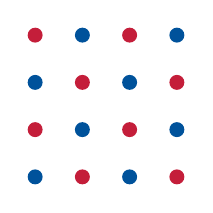
\begin{tikzpicture}[scale=.60]
      \foreach \x in {0,...,3}{
        \foreach \y in {0,...,3}{
          \pgfmathparse{mod(\x+\y,2)==0 ? "JapanBlue" : "ChinaRed"}
          \edef\cc{\pgfmathresult}
          \fill[\cc] (\x,\y) circle (4.5pt);
        }
      }
    \end{tikzpicture}
    \par\jp{イオン結晶}
    \par\scriptsize 正負イオンの三次元配列

    \column{.24\textwidth}
    \centering
    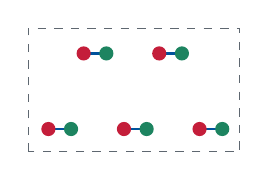
\begin{tikzpicture}[scale=.64]
      \foreach \x/\y in {0/0,1.5/0,3/0,.7/1.5,2.2/1.5}{
        \draw[thick,JapanBlue] (\x,\y)--++(.45,0);
        \fill[ChinaRed] (\x,\y) circle (4pt);
        \fill[ChemGreen] (\x+.45,\y) circle (4pt);
      }
      \draw[dashed,GraphGray] (-.4,-.45) rectangle (3.8,2.0);
    \end{tikzpicture}
    \par\jp{分子結晶}
    \par\scriptsize 分子内は強く、分子間は弱い

    \column{.24\textwidth}
    \centering
    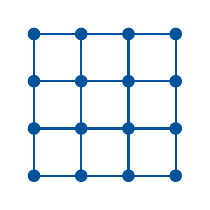
\begin{tikzpicture}[scale=.60]
      \foreach \x in {0,...,3}{
        \foreach \y in {0,...,3}{
          \fill[JapanBlue] (\x,\y) circle (3.8pt);
          \ifnum\x<3 \draw[JapanBlue,thick] (\x,\y)--(\x+1,\y);\fi
          \ifnum\y<3 \draw[JapanBlue,thick] (\x,\y)--(\x,\y+1);\fi
        }
      }
    \end{tikzpicture}
    \par\jp{共有結合の結晶}
    \par\scriptsize 結晶全体が結合網

    \column{.24\textwidth}
    \centering
    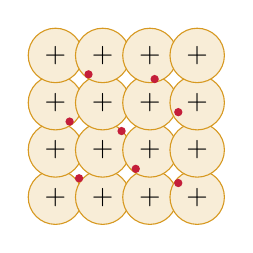
\begin{tikzpicture}[scale=.60]
      \foreach \x in {0,...,3}{
        \foreach \y in {0,...,3}{
          \node[circle,draw=Gold,fill=Gold!18,minimum size=5mm]
            at (\x,\y) {$+$};
        }
      }
      \foreach \x/\y in {.5/.4,1.7/.6,2.6/.3,.3/1.6,1.4/1.4,2.6/1.8,.7/2.6,2.1/2.5}
        \fill[ChinaRed] (\x,\y) circle (2.5pt);
    \end{tikzpicture}
    \par\jp{金属結晶}
    \par\scriptsize 自由電子が結晶内を移動
  \end{columns}
\end{frame}

\begin{frame}{イオン結晶：強いが、ずれるともろい}
  \begin{columns}[T,onlytextwidth]
    \column{.47\textwidth}
    \begin{block}{性質の理由}
      \begin{itemize}
        \item 正負イオン間の強い静電気力
        \item 固体ではイオンが格子点に固定
        \item 融解または水に溶けるとイオンが移動可能
      \end{itemize}
    \end{block}
    \[
      \chem{NaCl(s)}\ \text{不導体}
      \qquad
      \chem{NaCl(l)}\ \text{導体}
    \]
    \column{.49\textwidth}
    \centering
    \begin{tikzpicture}[scale=.72,>=Latex]
      \foreach \x in {0,...,4}{
        \foreach \y in {0,...,2}{
          \pgfmathparse{mod(\x+\y,2)==0 ? "JapanBlue" : "ChinaRed"}
          \edef\cc{\pgfmathresult}
          \fill[\cc] (\x,\y) circle (5pt);
          \node[white,font=\tiny\bfseries] at (\x,\y)
            {\ifnum\numexpr\x+\y\relax=0 +\fi};
        }
      }
      \draw[->,very thick,GraphGray] (1.8,3.0)--(3.2,3.0)
        node[midway,above]{ずれる};
      \foreach \x in {0,...,4}{
        \foreach \y in {0,...,1}{
          \pgfmathparse{mod(\x+\y,2)==0 ? "JapanBlue" : "ChinaRed"}
          \edef\cc{\pgfmathresult}
          \fill[\cc] (\x+5.4,\y+1) circle (5pt);
        }
      }
      \foreach \x in {0,...,4}{
        \pgfmathparse{mod(\x,2)==0 ? "ChinaRed" : "JapanBlue"}
        \edef\cc{\pgfmathresult}
        \fill[\cc] (\x+5.9,0) circle (5pt);
      }
      \draw[<->,ChinaRed,very thick] (6.0,.6)--(6.0,.25);
      \node[align=center] at (6.9,-.7){同符号が近づき\\反発して割れる};
    \end{tikzpicture}
  \end{columns}
\end{frame}

\begin{frame}{分子結晶：分子間力が性質を決める}
  \begin{columns}[T,onlytextwidth]
    \column{.48\textwidth}
    \begin{block}{二つの“力”を分ける}
      \begin{itemize}
        \item 分子内：共有結合（強い）
        \item 分子間：分子間力（比較的弱い）
      \end{itemize}
    \end{block}
    融解や沸騰では、通常\key{共有結合を切らず}、
    分子間の距離を広げる。
    \column{.48\textwidth}
    \begin{exampleblock}{沸点を高くする要因}
      \begin{itemize}
        \item 分子量が大きい
        \item 分子の極性が大きい
        \item 水素結合が存在する
      \end{itemize}
    \end{exampleblock}
    例：$\chem{H_2O}$、$\chem{NH_3}$、$\chem{HF}$。
  \end{columns}

  \vfill
  \centering
  \begin{tikzpicture}[>=Latex]
    \node[draw,rounded corners,fill=SoftBlue] (a) {$\chem{H-O-H}$};
    \node[draw,rounded corners,fill=SoftBlue,right=18mm of a] (b) {$\chem{H-O-H}$};
    \draw[densely dashed,very thick,ChinaRed] (a)--(b)
      node[midway,above]{水素結合};
  \end{tikzpicture}
\end{frame}

\begin{frame}{共有結合の結晶：結晶全体が一つの網目}
  \begin{columns}[T,onlytextwidth]
    \column{.48\textwidth}
    \begin{block}{代表例}
      \begin{itemize}
        \item ダイヤモンド $\chem C$
        \item 二酸化ケイ素 $\chem{SiO_2}$
        \item ケイ素 $\chem{Si}$
        \item 炭化ケイ素 $\chem{SiC}$
      \end{itemize}
    \end{block}
    多数の共有結合を切らないと融解しないため、
    非常に高い融点をもつ。
    \column{.48\textwidth}
    \begin{alertblock}{黒鉛は重要な例外}
      黒鉛では炭素原子が層状に結合し、各層に自由に動ける電子がある。
      そのため\key{電気を通す}。
    \end{alertblock}
    \begin{itemize}
      \item ダイヤモンド：硬い、不導体
      \item 黒鉛：柔らかい、導体
    \end{itemize}
  \end{columns}
\end{frame}

\begin{frame}{金属結晶：自由電子による性質}
  \begin{columns}[T,onlytextwidth]
    \column{.50\textwidth}
    \begin{block}{金属結合}
      金属原子が価電子を結晶全体に共有し、
      金属陽イオンと\jp{自由電子}の間の静電気力で結合する。
    \end{block}
    \begin{itemize}
      \item 電気伝導性・熱伝導性が高い
      \item 展性（薄く広げられる）
      \item 延性（細く伸ばせる）
      \item 金属光沢
    \end{itemize}
    \column{.46\textwidth}
    \centering
    \begin{tikzpicture}[scale=.75,>=Latex]
      \foreach \x in {0,...,4}{
        \foreach \y in {0,...,3}{
          \node[circle,draw=Gold,fill=Gold!20,minimum size=7mm]
            at (\x,\y) {$+$};
        }
      }
      \foreach \x/\y in {.5/.4,1.7/.6,2.9/.35,3.6/.8,.3/1.6,1.3/1.4,2.4/1.8,3.5/1.5,.6/2.6,2/2.5,3.2/2.7}
        \fill[ChinaRed] (\x,\y) circle (3pt);
      \draw[->,very thick,JapanBlue] (.2,-.65)--(3.8,-.65)
        node[midway,below]{電場で電子が移動};
    \end{tikzpicture}
  \end{columns}
\end{frame}

\begin{frame}{溶解性：「似たものどうしは溶けやすい」}
  \begin{columns}[T,onlytextwidth]
    \column{.47\textwidth}
    \begin{block}{極性溶媒}
      水のように極性をもつ溶媒は
      \begin{itemize}
        \item イオン性物質
        \item 極性分子
      \end{itemize}
      を溶かしやすい。
    \end{block}
    \column{.47\textwidth}
    \begin{exampleblock}{無極性溶媒}
      ヘキサンのような無極性溶媒は
      \begin{itemize}
        \item ヨウ素 $\chem{I_2}$
        \item 油脂
      \end{itemize}
      などの無極性物質を溶かしやすい。
    \end{exampleblock}
  \end{columns}

  \begin{alertblock}{注意}
    これは傾向を示す経験則。結晶格子の強さ、分子間力、温度なども
    実際の溶解度に影響する。
  \end{alertblock}
\end{frame}

\begin{frame}{例題1｜結晶の種類：問題}
  \def\exq{
    ある固体 X は融点が高く、固体では電気を通さないが、
    融解すると電気を通す。X の結晶の種類を答え、
    導電性が変化する理由を説明せよ。
  }
  \only<1>{\vfill\questioncard{\exq}\vfill}
  \only<2>{
    \questioncard{\exq}
    \vfill
    \answercard{
      \ans{イオン結晶。}
      固体では陽イオンと陰イオンが格子点に固定されている。
      融解するとイオンが移動でき、電荷を運ぶため電気を通す。
    }
  }
\end{frame}

\begin{frame}{例題2｜電気伝導性：問題}
  \def\exq{
    次のうち、通常の状態で電気を通すものをすべて選べ。\quad
    (1) 固体 NaCl \quad
    (2) 溶融 NaCl \quad
    (3) Cu \quad
    (4) ダイヤモンド \quad
    (5) 黒鉛
  }
  \only<1>{\vfill\questioncard{\exq}\vfill}
  \only<2>{
    \questioncard{\exq}
    \vfill
    \answercard{
      \ans{(2)、(3)、(5)。}
      溶融 NaCl ではイオン、Cu では自由電子、黒鉛では層内の電子が
      電荷を運ぶ。固体 NaCl とダイヤモンドには移動可能な荷電粒子がない。
    }
  }
\end{frame}

\begin{frame}{例題3｜沸点の比較：問題}
  \def\exq{
    $\chem{CH_4}$ と $\chem{H_2O}$ はどちらも小さな分子であるが、
    $\chem{H_2O}$ の沸点は著しく高い。その主な理由を、
    分子間力の名称を用いて説明せよ。
  }
  \only<1>{\vfill\questioncard{\exq}\vfill}
  \only<2>{
    \questioncard{\exq}
    \vfill
    \answercard{
      $\chem{H_2O}$ 分子間には強い\jp{水素結合}が働く。
      $\chem{CH_4}$ は無極性分子で、主に弱い分散力が働く。
      したがって水分子を互いに引き離すために、より多くのエネルギーが必要。
    }
  }
\end{frame}

% ================================================================
\section{相対原子質量・原子量・分子量・式量}

\begin{frame}{なぜ「相対質量」を使うのか}
  原子一個の実際の質量は非常に小さい。
  そこで、炭素12原子一個の質量の $1/12$ を基準 1 とする。

  \[
    \boxed{
      \text{相対原子質量}
      =
      \frac{\text{ある原子一個の質量}}
      {\frac1{12}\times\text{炭素12原子一個の質量}}
    }
  \]

  \begin{columns}[c,onlytextwidth]
    \column{.52\textwidth}
    \begin{block}{重要}
      相対質量は比なので\key{単位をもたない}。
      炭素12の相対原子質量は定義によりちょうど 12。
    \end{block}
    \column{.44\textwidth}
    \centering
    \begin{tikzpicture}[scale=.8]
      \draw[thick] (-2.4,0)--(2.4,0);
      \draw[fill=SoftBlue,thick] (-2,-.2) rectangle (-.8,.6);
      \node at (-1.4,.2) {$^{12}\chem C$};
      \foreach \x in {0,...,11}
        \fill[ChinaRed] ({-.45+.25*mod(\x,6)},{-.1+.35*int(\x/6)}) circle (2.5pt);
      \node[align=center] at (.3,-.9){12等分した\\一つを基準1};
    \end{tikzpicture}
  \end{columns}
\end{frame}

\begin{frame}{相対原子質量と原子量の違い}
  \begin{columns}[T,onlytextwidth]
    \column{.48\textwidth}
    \begin{block}{相対原子質量}
      特定の\key{一種類の同位体原子}の相対質量。
      \[
        ^{35}\chem{Cl}\approx34.97,\qquad
        ^{37}\chem{Cl}\approx36.97
      \]
    \end{block}
    \column{.48\textwidth}
    \begin{exampleblock}{原子量（げんしりょう）}
      元素中の各同位体の相対原子質量を、存在比で加重平均した値。
      \[
        \boxed{
        A_{\rm r}=\sum
        (\text{同位体の相対質量})
        \times(\text{存在比})
        }
      \]
    \end{exampleblock}
  \end{columns}

  \vfill
  \centering
  \key{质量数是整数；相对原子质量和原子量通常不是整数。}
\end{frame}

\begin{frame}{原子量は同位体存在比の加重平均}
  \begin{columns}[T,onlytextwidth]
    \column{.52\textwidth}
    天然塩素を簡略化して
    \[
      ^{35}\chem{Cl}:75.0\%,
      \qquad
      ^{37}\chem{Cl}:25.0\%
    \]
    とすると
    \[
      A_{\rm r}(\chem{Cl})
      =35.0\times0.750+37.0\times0.250
      =35.5.
    \]
    \column{.44\textwidth}
    \centering
    \begin{tikzpicture}[x=.72cm,y=.038cm,>=Latex]
      \draw[->] (0,0)--(5.1,0) node[right]{相対質量};
      \draw[->] (0,0)--(0,85) node[above]{存在比};
      \fill[JapanBlue] (1.0,0) rectangle (2.0,75);
      \fill[ChinaRed] (3.0,0) rectangle (4.0,25);
      \node[below] at (1.5,0){35};
      \node[below] at (3.5,0){37};
      \node[left] at (0,75){75\%};
      \node[left] at (0,25){25\%};
    \end{tikzpicture}
  \end{columns}

  \begin{alertblock}{存在比の扱い}
    計算では $75.0\%=0.750$ のように小数へ直す。
    各存在比の合計は 1（または 100\%）。
  \end{alertblock}
\end{frame}

\begin{frame}{分子量（ぶんしりょう）}
  分子をつくるすべての原子の原子量を合計する。
  \[
    \boxed{
      M_{\rm r}
      =
      \sum(\text{各元素の原子量}\times\text{原子数})
    }
  \]

  \begin{columns}[T,onlytextwidth]
    \column{.48\textwidth}
    \begin{block}{水}
      \[
        M_{\rm r}(\chem{H_2O})
        =1.0\times2+16.0
        =18.0
      \]
    \end{block}
    \column{.48\textwidth}
    \begin{exampleblock}{二酸化炭素}
      \[
        M_{\rm r}(\chem{CO_2})
        =12.0+16.0\times2
        =44.0
      \]
    \end{exampleblock}
  \end{columns}

  \vfill
  \centering
  分子量也是相对值，\key{没有单位}。
\end{frame}

\begin{frame}{式量（しきりょう）}
  イオン結晶や共有結合の結晶には独立した分子がない。
  そこで、組成式中の原子の原子量の合計を\jp{式量}という。

  \begin{columns}[T,onlytextwidth]
    \column{.48\textwidth}
    \begin{block}{塩化ナトリウム}
      \[
        \chem{NaCl}:
        \quad23.0+35.5=\boxed{58.5}
      \]
    \end{block}
    \column{.48\textwidth}
    \begin{exampleblock}{炭酸カルシウム}
      \[
        \chem{CaCO_3}:
        \quad40.0+12.0+16.0\times3
        =\boxed{100}
      \]
    \end{exampleblock}
  \end{columns}

  \begin{alertblock}{分子量か式量か}
    $\chem{H_2O}$、$\chem{CO_2}$ のような分子性物質は分子量。
    $\chem{NaCl}$、$\chem{CaCO_3}$、$\chem{SiO_2}$ は式量。
  \end{alertblock}
\end{frame}

\begin{frame}{相対質量とモル質量を区別する}
  \small
  \begin{tabular}{>{\bfseries\color{JapanBlue}}p{.22\linewidth}
                  p{.30\linewidth}p{.33\linewidth}}
    \toprule
    量 & 意味 & 単位\\
    \midrule
    原子量 &
    元素の相対的な平均質量 &
    なし\\[.6em]
    分子量・式量 &
    分子式・組成式に含まれる相対質量の和 &
    なし\\[.6em]
    モル質量 $M$ &
    物質 1 mol あたりの質量 &
    $\mathrm{g/mol}$\\
    \bottomrule
  \end{tabular}

  \vfill
  \begin{block}{数値上の関係}
    \[
      M_{\rm r}(\chem{H_2O})=18.0
      \qquad\Longleftrightarrow\qquad
      M(\chem{H_2O})=18.0\unit{g/mol}
    \]
    数值相同，但物理意义和单位不同。
  \end{block}
\end{frame}

\begin{frame}{例題4｜原子量：問題}
  \def\exq{
    ある元素 X には相対原子質量 10.0 と 11.0 の同位体があり、
    存在比はそれぞれ 20.0\%、80.0\% である。X の原子量を求めよ。
  }
  \only<1>{\vfill\questioncard{\exq}\vfill}
  \only<2>{
    \questioncard{\exq}
    \vfill
    \answercard{
      \[
        A_{\rm r}(\chem X)
        =10.0\times0.200+11.0\times0.800
        =2.00+8.80
        =\boxed{10.8}
      \]
      两种存在比相加为 1，结果必须位于 10.0 和 11.0 之间。
    }
  }
\end{frame}

\begin{frame}{例題5｜存在比の逆算：問題}
  \def\exq{
    元素 Y は相対原子質量 24.0 と 26.0 の二同位体からなり、
    原子量は 24.4 である。質量 26.0 の同位体の存在比を求めよ。
  }
  \only<1>{\vfill\questioncard{\exq}\vfill}
  \only<2>{
    \questioncard{\exq}
    \vfill
    \answercard{
      質量 26.0 の存在比を $x$ とすると
      \[
        24.0(1-x)+26.0x=24.4.
      \]
      \[
        2.0x=0.4
        \quad\Rightarrow\quad
        x=0.20=\boxed{20\%}.
      \]
    }
  }
\end{frame}

\begin{frame}{例題6｜分子量：問題}
  \def\exq{
    原子量を H=1.0、C=12.0、O=16.0 とする。
    エタノール $\chem{C_2H_6O}$ の分子量を求めよ。
  }
  \only<1>{\vfill\questioncard{\exq}\vfill}
  \only<2>{
    \questioncard{\exq}
    \vfill
    \answercard{
      \[
        M_{\rm r}
        =12.0\times2+1.0\times6+16.0
        =24.0+6.0+16.0
        =\boxed{46.0}
      \]
      下付き数字を各元素的原子数として逐项相加。
    }
  }
\end{frame}

\begin{frame}{例題7｜式量：問題}
  \def\exq{
    原子量を Al=27.0、S=32.0、O=16.0 とする。
    硫酸アルミニウム $\chem{Al_2(SO_4)_3}$ の式量を求めよ。
  }
  \only<1>{\vfill\questioncard{\exq}\vfill}
  \only<2>{
    \questioncard{\exq}
    \vfill
    \answercard{
      括弧の外の 3 を、S と O$_4$ の両方に掛ける。
      \[
        27.0\times2+
        (32.0+16.0\times4)\times3
        =54.0+96.0\times3
        =\boxed{342}
      \]
    }
  }
\end{frame}

\begin{frame}{例題8｜質量百分率：問題}
  \def\exq{
    $\chem{CaCO_3}$ の式量を 100 とする。
    $\chem{CaCO_3}$ 中の酸素の質量百分率を求めよ。
  }
  \only<1>{\vfill\questioncard{\exq}\vfill}
  \only<2>{
    \questioncard{\exq}
    \vfill
    \answercard{
      組成式一単位中の酸素の相対質量は
      \[
        16.0\times3=48.0.
      \]
      \[
        \frac{48.0}{100}\times100
        =\boxed{48.0\%}
      \]
      这里计算的是化合物中元素的质量组成，不是溶液浓度。
    }
  }
\end{frame}

% ================================================================
\section{物質量の定義と関連計算}

\begin{frame}{物質量（ぶっしつりょう）と mol}
  \begin{block}{定義}
    \jp{物質量} $n$ は、物質を構成する粒子の個数を表す量。
    単位は\jp{モル（mol）}。
  \end{block}

  \[
    \boxed{
      1\unit{mol}
      =6.02214076\times10^{23}\ \text{個}
    }
  \]
  高校計算では多くの場合
  \[
    N_{\rm A}=6.02\times10^{23}\unit{mol^{-1}}
  \]
  を用いる。

  \begin{alertblock}{粒子を必ず明示}
    原子、分子、イオン、電子、式単位のどれを数えているかを書く。
    例：1 mol の $\chem{NaCl}$ には Na$^+$ も Cl$^-$ も各 1 mol。
  \end{alertblock}
\end{frame}

\begin{frame}{1 mol は「化学の一箱」}
  \begin{columns}[c,onlytextwidth]
    \column{.42\textwidth}
    \centering
    \begin{tikzpicture}[scale=.9]
      \draw[fill=SoftBlue,thick,rounded corners]
        (-2,-1.4) rectangle (2,1.4);
      \node[font=\Large\bfseries,JapanBlue] at (0,.85){1 mol};
      \node[font=\large] at (0,.15){$6.02\times10^{23}$ 個};
      \foreach \x/\y in {-1.3/-.7,-.7/-.75,-.1/-.68,.5/-.72,1.1/-.7}
        \fill[ChinaRed] (\x,\y) circle (3.5pt);
    \end{tikzpicture}
    \column{.54\textwidth}
    \begin{itemize}
      \item 卵 1 dozen = 12 個
      \item 粒子 1 mol = $N_{\rm A}$ 個
    \end{itemize}
    \begin{block}{个数与 mol 的关系}
      \[
        \boxed{N=nN_{\rm A}}
        \qquad
        \boxed{n=\frac{N}{N_{\rm A}}}
      \]
    \end{block}
    “mol”不是粒子的种类，而是\key{计数单位}。
  \end{columns}
\end{frame}

\begin{frame}{モル質量と質量}
  物質 1 mol の質量を\jp{モル質量} $M$ という。
  \[
    \boxed{n=\frac{m}{M}}
    \qquad
    \boxed{m=nM}
  \]

  \begin{columns}[T,onlytextwidth]
    \column{.48\textwidth}
    \begin{block}{例：水}
      \[
        M(\chem{H_2O})=18.0\unit{g/mol}
      \]
      \[
        36.0\unit g
        \Rightarrow
        n=\frac{36.0}{18.0}=2.00\unit{mol}
      \]
    \end{block}
    \column{.48\textwidth}
    \begin{alertblock}{単位で確認}
      \[
        \frac{\mathrm g}{\mathrm{g/mol}}
        =\mathrm{mol}
      \]
      单位能够帮助检查乘除方向是否写反。
    \end{alertblock}
  \end{columns}
\end{frame}

\begin{frame}{mol 換算マップ}
  \centering
  \begin{tikzpicture}[
    >=Latex,node distance=17mm,
    box/.style={
      draw,rounded corners=2mm,minimum width=31mm,
      minimum height=13mm,align=center,font=\bfseries
    }]
    \node[box,draw=JapanBlue,fill=SoftBlue] (mol) {物質量\\$n$ [mol]};
    \node[box,draw=ChinaRed,fill=SoftRed,left=of mol] (mass) {質量\\$m$ [g]};
    \node[box,draw=ChemGreen,fill=SoftGreen,right=of mol] (num) {粒子数\\$N$ [個]};
    \node[box,draw=Gold,fill=Gold!15,below=of mol] (gas) {気体体積\\$V$ [L]};
    \draw[<->,very thick,JapanBlue] (mass)--(mol)
      node[midway,above] {$\div M$}
      node[midway,below] {$\times M$};
    \draw[<->,very thick,ChemGreen] (mol)--(num)
      node[midway,above] {$\times N_{\rm A}$}
      node[midway,below] {$\div N_{\rm A}$};
    \draw[<->,very thick,Gold] (mol)--(gas)
      node[midway,right] {$\times V_{\rm m}$}
      node[midway,left] {$\div V_{\rm m}$};
  \end{tikzpicture}

  \vfill
  \begin{alertblock}{中心に mol を置く}
    质量、粒子数、气体体积之间不要直接换算。
    先换成 mol，再去目标单位。
  \end{alertblock}
\end{frame}

\begin{frame}{気体のモル体積}
  \begin{block}{標準状態}
    $0^\circ\mathrm C$、$1.013\times10^5\unit{Pa}$ では、
    理想気体 1 mol の体積は
    \[
      \boxed{V_{\rm m}=22.4\unit{L/mol}}.
    \]
  \end{block}

  \[
    \boxed{V=nV_{\rm m}}
    \qquad
    \boxed{n=\frac{V}{V_{\rm m}}}
  \]

  \begin{columns}[T,onlytextwidth]
    \column{.48\textwidth}
    \begin{exampleblock}{同温・同圧}
      相同温度和压力下，等体积气体含有相同分子数。
    \end{exampleblock}
    \column{.48\textwidth}
    \begin{alertblock}{条件を必ず確認}
      22.4 L/mol は標準状態だけ。温度・圧力が変われば体積も変わる。
    \end{alertblock}
  \end{columns}
\end{frame}

\begin{frame}{化学反応式と mol 比}
  \begin{block}{係数は粒子数比であり、mol 比}
    \[
      2\chem{H_2}+\chem{O_2}
      \longrightarrow
      2\chem{H_2O}
    \]
    \[
      n(\chem{H_2}):n(\chem{O_2}):n(\chem{H_2O})
      =2:1:2.
    \]
  \end{block}

  \reasonflow{与えられた量を mol へ}{係数比で目的物質の mol}{質量・体積・個数へ}

  \begin{alertblock}{係数と下付き数字}
    係数は物質全体の個数・mol 数を変える。
    下付き数字は一個の分子内の原子数を示し、勝手に変えてはいけない。
  \end{alertblock}
\end{frame}

\begin{frame}{限界反応物（げんかいはんのうぶつ）}
  複数の反応物が与えられたとき、先に使い切る物質を
  \jp{限界反応物} \en{limiting reagent} という。

  \begin{columns}[T,onlytextwidth]
    \column{.47\textwidth}
    \begin{block}{判断法1}
      各反応物について
      \[
        \frac{\text{物質量}}{\text{反応係数}}
      \]
      を比較し、小さいものが限界反応物。
    \end{block}
    \column{.49\textwidth}
    \begin{exampleblock}{判断法2}
      一方を完全に反応させるために必要な他方の量を計算し、
      实际量と比較する。
    \end{exampleblock}
  \end{columns}

  \vfill
  \centering
  \key{生成物の量は、限界反応物によって決まる。}
\end{frame}

\begin{frame}{例題9｜粒子数：問題}
  \def\exq{
    $0.250\unit{mol}$ の $\chem{CO_2}$ に含まれる
    (1) $\chem{CO_2}$ 分子の個数、
    (2) 酸素原子の個数を求めよ。
    $N_{\rm A}=6.02\times10^{23}\unit{mol^{-1}}$ とする。
  }
  \only<1>{\vfill\questioncard{\exq}\vfill}
  \only<2>{
    \questioncard{\exq}
    \vfill
    \answercard{
      \[
        N(\chem{CO_2})
        =0.250\times6.02\times10^{23}
        =\boxed{1.51\times10^{23}\ \text{個}}.
      \]
      一分子含 2 个氧原子，因此
      \[
        N(\chem O)=2N(\chem{CO_2})
        =\boxed{3.01\times10^{23}\ \text{個}}.
      \]
    }
  }
\end{frame}

\begin{frame}{例題10｜質量と mol：問題}
  \def\exq{
    $\chem{CaCO_3}$ のモル質量を $100\unit{g/mol}$ とする。
    $25.0\unit g$ の $\chem{CaCO_3}$ の物質量と式単位の個数を求めよ。
  }
  \only<1>{\vfill\questioncard{\exq}\vfill}
  \only<2>{
    \questioncard{\exq}
    \vfill
    \answercard{
      \[
        n=\frac{m}{M}=\frac{25.0}{100}
        =\boxed{0.250\unit{mol}}.
      \]
      \[
        N=nN_{\rm A}
        =0.250\times6.02\times10^{23}
        =\boxed{1.51\times10^{23}\ \text{個}}.
      \]
    }
  }
\end{frame}

\begin{frame}{例題11｜気体体積：問題}
  \def\exq{
    標準状態で $11.2\unit L$ の酸素 $\chem{O_2}$ がある。
    (1) 物質量、(2) 分子数、(3) 質量を求めよ。
    $M(\chem{O_2})=32.0\unit{g/mol}$。
  }
  \only<1>{\vfill\questioncard{\exq}\vfill}
  \only<2>{
    \questioncard{\exq}
    \vfill
    \answercard{
      \[
        n=\frac{11.2}{22.4}
        =\boxed{0.500\unit{mol}}.
      \]
      \[
        N=0.500N_{\rm A}
        =\boxed{3.01\times10^{23}\ \text{個}},
        \qquad
        m=0.500\times32.0
        =\boxed{16.0\unit g}.
      \]
    }
  }
\end{frame}

\begin{frame}{例題12｜反応式の係数比：問題}
  \def\exq{
    $2\chem{H_2}+\chem{O_2}\rightarrow2\chem{H_2O}$ において、
    $\chem{O_2}$ $0.500\unit{mol}$ が十分な $\chem{H_2}$ と完全に反応する。
    生成する水の物質量と質量を求めよ。
  }
  \only<1>{\vfill\questioncard{\exq}\vfill}
  \only<2>{
    \questioncard{\exq}
    \vfill
    \answercard{
      係数比 $\chem{O_2}:\chem{H_2O}=1:2$ より
      \[
        n(\chem{H_2O})
        =0.500\times2
        =\boxed{1.00\unit{mol}}.
      \]
      \[
        m=nM=1.00\times18.0
        =\boxed{18.0\unit g}.
      \]
    }
  }
\end{frame}

\begin{frame}{例題13｜限界反応物：問題}
  \def\exq{
    $2\chem{H_2}+\chem{O_2}\rightarrow2\chem{H_2O}$ において、
    $\chem{H_2}$ $3.0\unit{mol}$ と $\chem{O_2}$ $2.0\unit{mol}$ を反応させる。
    限界反応物、生成する水の物質量、余る反応物の物質量を求めよ。
  }
  \only<1>{\vfill\questioncard{\exq}\vfill}
  \only<2>{
    \questioncard{\exq}
    \vfill
    \answercard{
      \[
        \frac{3.0}{2}=1.5,
        \qquad
        \frac{2.0}{1}=2.0
      \]
      より、\ans{$\chem{H_2}$ が限界反応物。}
      係数比から水は $3.0\unit{mol}$ 生じ、
      消費する $\chem{O_2}$ は $1.5\unit{mol}$。
      \[
        n_{\rm remain}(\chem{O_2})
        =2.0-1.5
        =\boxed{0.5\unit{mol}}.
      \]
    }
  }
\end{frame}

% ================================================================
\section{溶液の濃度}

\begin{frame}{溶液・溶質・溶媒}
  \begin{columns}[c,onlytextwidth]
    \column{.47\textwidth}
    \centering
    \begin{tikzpicture}[scale=.85]
      \draw[very thick,JapanBlue]
        (-2,2.5)--(-1.55,-1.4)--(1.55,-1.4)--(2,2.5);
      \fill[SoftBlue] (-1.75,1.3)--(-1.55,-1.4)--(1.55,-1.4)--(1.75,1.3)--cycle;
      \foreach \x/\y in {-1.2/.6,-.5/.9,.1/.5,.8/.85,1.2/.2,-.9/-.4,-.2/-.7,.6/-.4}
        \fill[ChinaRed] (\x,\y) circle (3.2pt);
      \node[JapanBlue] at (0,1.7){溶媒};
      \node[ChinaRed] at (0,-1.9){赤点：溶質粒子};
    \end{tikzpicture}
    \column{.49\textwidth}
    \begin{block}{用語}
      \begin{itemize}
        \item \jp{溶質（ようしつ）}：溶けている物質
        \item \jp{溶媒（ようばい）}：溶かす物質
        \item \jp{溶液（ようえき）}：均一な混合物
      \end{itemize}
    \end{block}
    \[
      m_{\rm solution}
      =m_{\rm solute}+m_{\rm solvent}
    \]
    溶液の体積は、一般に各成分の体積の単純和とは限らない。
  \end{columns}
\end{frame}

\begin{frame}{質量パーセント濃度}
  \begin{block}{定義}
    \[
      \boxed{
        w
        =
        \frac{\text{溶質の質量}}
             {\text{溶液の質量}}
        \times100\%
      }
    \]
  \end{block}

  \begin{columns}[T,onlytextwidth]
    \column{.47\textwidth}
    \begin{exampleblock}{分母に注意}
      \[
        m_{\rm solution}
        =m_{\rm solute}+m_{\rm solvent}.
      \]
      分母不是溶剂质量。
    \end{exampleblock}
    \column{.49\textwidth}
    \begin{alertblock}{単位}
      分子と分母は同じ質量単位を使う。
      g 同士でも kg 同士でも比は同じ。
    \end{alertblock}
  \end{columns}

  \centering
  100 g の溶液中に溶質が何 g あるかを表す濃度。
\end{frame}

\begin{frame}{モル濃度（モルのうど）}
  \begin{block}{定義 \en{molar concentration}}
    \[
      \boxed{
        c=\frac{n_{\rm solute}}{V_{\rm solution}}
      }
      \qquad
      [c]=\mathrm{mol/L}
    \]
  \end{block}

  \begin{columns}[T,onlytextwidth]
    \column{.48\textwidth}
    \begin{itemize}
      \item 分子：溶質の物質量
      \item 分母：\key{溶液全体の体積}
      \item mL は L に直す
    \end{itemize}
    \column{.48\textwidth}
    \begin{exampleblock}{体積換算}
      \[
        250\unit{mL}=0.250\unit L
      \]
      \[
        n=cV
      \]
      $V$ を L で代入すると mol が得られる。
    \end{exampleblock}
  \end{columns}
\end{frame}

\begin{frame}{質量モル濃度}
  \begin{block}{定義 \en{molality}}
    \[
      \boxed{
        b=
        \frac{n_{\rm solute}}
             {m_{\rm solvent}[\mathrm{kg}]}
      }
      \qquad
      [b]=\mathrm{mol/kg}
    \]
  \end{block}

  \begin{columns}[T,onlytextwidth]
    \column{.48\textwidth}
    \begin{itemize}
      \item 分子：溶質の物質量
      \item 分母：\key{溶媒だけ}の質量
      \item g ではなく kg に直す
    \end{itemize}
    \column{.48\textwidth}
    \begin{alertblock}{モル濃度との違い}
      モル濃度の分母は\key{溶液の体積 L}。
      質量モル濃度の分母は\key{溶媒の質量 kg}。
    \end{alertblock}
  \end{columns}
\end{frame}

\begin{frame}{三種類の濃度を並べて比較}
  \small
  \begin{tabular}{>{\bfseries\color{JapanBlue}}p{.20\linewidth}
                  p{.23\linewidth}p{.21\linewidth}p{.17\linewidth}}
    \toprule
    濃度 & 分子 & 分母 & 単位\\
    \midrule
    質量パーセント濃度 &
    溶質の質量 &
    溶液の質量 &
    \%\\[.8em]
    モル濃度 &
    溶質の物質量 &
    溶液の体積 &
    mol/L\\[.8em]
    質量モル濃度 &
    溶質の物質量 &
    溶媒の質量 &
    mol/kg\\
    \bottomrule
  \end{tabular}

  \vfill
  \begin{alertblock}{温度の影響}
    体積は温度で変化するのでモル濃度も変化しうる。
    質量に基づく質量百分率と質量モル濃度は、蒸発などがなければ
    温度変化の影響を受けにくい。
  \end{alertblock}
\end{frame}

\begin{frame}{希釈（きしゃく）}
  水を加えても、溶質を失わなければ溶質の物質量は保存される。
  \[
    \boxed{c_1V_1=c_2V_2}
  \]

  \begin{columns}[c,onlytextwidth]
    \column{.44\textwidth}
    \centering
    \begin{tikzpicture}[scale=.72,>=Latex]
      \draw[thick] (-2,2.6)--(-1.6,-1.2)--(1.6,-1.2)--(2,2.6);
      \fill[JapanBlue!40] (-1.75,1.4)--(-1.6,-1.2)--(1.6,-1.2)--(1.75,1.4)--cycle;
      \foreach \x/\y in {-1/.7,-.3/.9,.4/.6,1/.8,-.7/-.2,.1/-.5,.8/-.1}
        \fill[ChinaRed] (\x,\y) circle (3pt);
      \node at (0,-1.7){濃い：$c_1,V_1$};
    \end{tikzpicture}
    \column{.08\textwidth}
    \centering
    \Large$\Longrightarrow$
    \column{.44\textwidth}
    \centering
    \begin{tikzpicture}[scale=.72]
      \draw[thick] (-2,2.6)--(-1.6,-1.2)--(1.6,-1.2)--(2,2.6);
      \fill[JapanBlue!18] (-1.9,2.2)--(-1.6,-1.2)--(1.6,-1.2)--(1.9,2.2)--cycle;
      \foreach \x/\y in {-1/1.1,-.3/1.5,.4/.8,1/1.4,-.7/-.2,.1/-.5,.8/-.1}
        \fill[ChinaRed] (\x,\y) circle (3pt);
      \node at (0,-1.7){薄い：$c_2,V_2$};
    \end{tikzpicture}
  \end{columns}

  \centering
  赤点の数（溶質量）は変わらず、体積だけ増える。
\end{frame}

\begin{frame}{質量百分率と密度からモル濃度へ}
  質量百分率 $w\%$、密度 $\rho\unit{g/mL}$、
  溶質のモル質量 $M\unit{g/mol}$ の溶液を考える。

  \begin{columns}[T,onlytextwidth]
    \column{.57\textwidth}
    溶液 1.00 L を仮定すると
    \[
      m_{\rm solution}
      =1000\rho\unit g.
    \]
    \[
      m_{\rm solute}
      =1000\rho\times\frac{w}{100}
      =10\rho w\unit g.
    \]
    \[
      c=\frac{10\rho w}{M}.
    \]
    \column{.39\textwidth}
    \begin{alertblock}{公式の条件}
      \[
        \boxed{c=\frac{10\rho w}{M}}
      \]
      ここで $w$ は 36.5 のような\key{百分率の数値}。
      $\rho$ は g/mL。
    \end{alertblock}
  \end{columns}
\end{frame}

\begin{frame}{例題14｜質量パーセント濃度：問題}
  \def\exq{
    食塩 $20.0\unit g$ を水 $80.0\unit g$ に溶かした。
    この食塩水の質量パーセント濃度を求めよ。
  }
  \only<1>{\vfill\questioncard{\exq}\vfill}
  \only<2>{
    \questioncard{\exq}
    \vfill
    \answercard{
      溶液の質量は
      \[
        20.0+80.0=100.0\unit g.
      \]
      \[
        w=\frac{20.0}{100.0}\times100
        =\boxed{20.0\%}.
      \]
      分母は水 80.0 g ではなく、溶液 100.0 g。
    }
  }
\end{frame}

\begin{frame}{例題15｜モル濃度：問題}
  \def\exq{
    $\chem{NaOH}$ $4.00\unit g$ を水に溶かし、
    溶液全体を $500\unit{mL}$ とした。
    $\chem{NaOH}$ のモル濃度を求めよ。
    $M(\chem{NaOH})=40.0\unit{g/mol}$。
  }
  \only<1>{\vfill\questioncard{\exq}\vfill}
  \only<2>{
    \questioncard{\exq}
    \vfill
    \answercard{
      \[
        n=\frac{4.00}{40.0}=0.100\unit{mol},
        \qquad
        V=0.500\unit L.
      \]
      \[
        c=\frac{n}{V}
        =\frac{0.100}{0.500}
        =\boxed{0.200\unit{mol/L}}.
      \]
    }
  }
\end{frame}

\begin{frame}{例題16｜質量モル濃度：問題}
  \def\exq{
    $\chem{NaCl}$ $5.85\unit g$ を水 $100\unit g$ に溶かした。
    質量モル濃度を求めよ。
    $M(\chem{NaCl})=58.5\unit{g/mol}$。
  }
  \only<1>{\vfill\questioncard{\exq}\vfill}
  \only<2>{
    \questioncard{\exq}
    \vfill
    \answercard{
      \[
        n(\chem{NaCl})=\frac{5.85}{58.5}
        =0.100\unit{mol}.
      \]
      水 $100\unit g=0.100\unit{kg}$ より
      \[
        b=\frac{0.100}{0.100}
        =\boxed{1.00\unit{mol/kg}}.
      \]
      分母使用的是水的质量，不是溶液总质量。
    }
  }
\end{frame}

\begin{frame}{例題17｜希釈：問題}
  \def\exq{
    $2.00\unit{mol/L}$ の溶液 $50.0\unit{mL}$ を水で薄め、
    $0.200\unit{mol/L}$ にした。希釈後の溶液全体の体積を求めよ。
  }
  \only<1>{\vfill\questioncard{\exq}\vfill}
  \only<2>{
    \questioncard{\exq}
    \vfill
    \answercard{
      \[
        c_1V_1=c_2V_2
      \]
      \[
        V_2=\frac{2.00\times50.0}{0.200}
        =\boxed{500\unit{mL}}.
      \]
      加えた水の体積を問われたなら
      $500-50.0=450\unit{mL}$。
    }
  }
\end{frame}

\begin{frame}{例題18｜密度を使う濃度換算：問題}
  \def\exq{
    質量パーセント濃度 36.5\%、密度
    $1.18\unit{g/mL}$ の塩酸がある。
    $\chem{HCl}$ のモル質量を $36.5\unit{g/mol}$ として、
    この塩酸のモル濃度を求めよ。
  }
  \only<1>{\vfill\questioncard{\exq}\vfill}
  \only<2>{
    \questioncard{\exq}
    \vfill
    \answercard{
      溶液 1.00 L を考える。
      \[
        m_{\rm solution}
        =1000\times1.18=1180\unit g.
      \]
      \[
        m(\chem{HCl})=1180\times0.365=430.7\unit g,
      \]
      \[
        c=\frac{430.7/36.5}{1.00}
        =\boxed{11.8\unit{mol/L}}.
      \]
    }
  }
\end{frame}

% ================================================================
\section{総合整理}

\begin{frame}{総合例題｜溶液から粒子数まで：問題}
  \def\exq{
    $0.500\unit{mol/L}$ の $\chem{NaCl}$ 水溶液
    $200\unit{mL}$ に含まれる
    (1) $\chem{NaCl}$ の物質量、
    (2) Na$^+$ の個数、
    (3) Cl$^-$ の個数を求めよ。
  }
  \only<1>{\vfill\questioncard{\exq}\vfill}
  \only<2>{
    \questioncard{\exq}
    \vfill
    \answercard{
      \[
        n=cV=0.500\times0.200
        =\boxed{0.100\unit{mol}}.
      \]
      $\chem{NaCl}\rightarrow\chem{Na^+}+\chem{Cl^-}$ より、
      両イオンも各 $0.100\unit{mol}$。
      \[
        N(\chem{Na^+})=N(\chem{Cl^-})
        =0.100\times6.02\times10^{23}
        =\boxed{6.02\times10^{22}\ \text{個}}.
      \]
    }
  }
\end{frame}

\begin{frame}{計算の共通手順}
  \begin{columns}[T,onlytextwidth]
    \column{.48\textwidth}
    \begin{block}{相対質量}
      \begin{enumerate}
        \item 同位体なら存在比を小数化
        \item 加重平均をとる
        \item 分子式・組成式の原子数を数える
      \end{enumerate}
    \end{block}
    \begin{block}{物質量}
      \begin{enumerate}
        \item 与えられた量を mol へ
        \item 必要なら反応係数比
        \item 求める単位へ戻す
      \end{enumerate}
    \end{block}
    \column{.48\textwidth}
    \begin{exampleblock}{濃度}
      \begin{enumerate}
        \item 溶質・溶媒・溶液を区別
        \item 分子と分母を定義通りに書く
        \item mL$\to$L、g$\to$kg を変換
        \item 密度があれば質量と体積を結ぶ
      \end{enumerate}
    \end{exampleblock}
    \begin{alertblock}{最后检查}
      数量级、有效数字、单位、粒子种类を確認する。
    \end{alertblock}
  \end{columns}
\end{frame}

\begin{frame}{重要語彙}
  \scriptsize
  \begin{tabular}{p{.27\linewidth}p{.26\linewidth}p{.35\linewidth}}
    \toprule
    日本語 & 読み方 & 中文・English\\
    \midrule
    構成粒子 & こうせいりゅうし & 构成粒子\\
    電気伝導性 & でんきでんどうせい & 导电性\\
    融点・沸点 & ゆうてん・ふってん & 熔点・沸点\\
    相対原子質量 & そうたいげんししつりょう & 相对原子质量\\
    原子量 & げんしりょう & 原子量 / atomic weight\\
    存在比 & そんざいひ & 丰度 / abundance\\
    分子量 & ぶんしりょう & 分子量\\
    式量 & しきりょう & 式量 / formula mass\\
    物質量 & ぶっしつりょう & 物质的量\\
    アボガドロ定数 & アボガドロていすう & 阿伏伽德罗常数\\
    モル質量 & モルしつりょう & 摩尔质量\\
    モル体積 & モルたいせき & 摩尔体积\\
    限界反応物 & げんかいはんのうぶつ & 限制反应物\\
    溶質・溶媒・溶液 & ようしつ・ようばい・ようえき & 溶质・溶剂・溶液\\
    質量パーセント濃度 & しつりょうパーセントのうど & 质量百分比浓度\\
    モル濃度 & モルのうど & 摩尔浓度 / molarity\\
    質量モル濃度 & しつりょうモルのうど & 质量摩尔浓度 / molality\\
    希釈 & きしゃく & 稀释 / dilution\\
    \bottomrule
  \end{tabular}
\end{frame}

\begin{frame}{公式マップ}
  \small
  \begin{columns}[T,onlytextwidth]
    \column{.48\textwidth}
    \begin{block}{相対質量・mol}
      \[
        A_{\rm r}=\sum m_i x_i
      \]
      \[
        n=\frac{m}{M},
        \qquad
        N=nN_{\rm A}
      \]
      \[
        V=nV_{\rm m}
        \quad(\text{標準状態 }V_{\rm m}=22.4\unit{L/mol})
      \]
    \end{block}
    \column{.48\textwidth}
    \begin{exampleblock}{濃度}
      \[
        w=\frac{m_{\rm solute}}{m_{\rm solution}}\times100\%
      \]
      \[
        c=\frac{n_{\rm solute}}{V_{\rm solution}},
        \qquad
        b=\frac{n_{\rm solute}}{m_{\rm solvent}[\mathrm{kg}]}
      \]
      \[
        c_1V_1=c_2V_2
      \]
    \end{exampleblock}
  \end{columns}
\end{frame}

\begin{frame}{授業内確認：問題}
  \def\exq{
    次の記述の正誤を判断し、誤りなら訂正せよ。
    \begin{enumerate}
      \item 分子量の単位は g/mol である。
      \item 1 mol の $\chem{CO_2}$ には酸素原子が 2 mol 含まれる。
      \item モル濃度の分母は溶媒の体積である。
      \item 質量モル濃度の分母は溶媒の質量 kg である。
      \item 希釈で溶質を失わなければ $cV$ は一定である。
    \end{enumerate}
  }
  \only<1>{\questioncard{\exq}}
  \only<2>{
    \questioncard{\exq}
    \vspace{.5em}
    \answercard{
      (1) 誤：分子量は無単位。g/mol はモル質量の単位。\quad
      (2) 正。\quad
      (3) 誤：溶液全体の体積。\quad
      (4) 正。\quad
      (5) 正。
    }
  }
\end{frame}

\begin{frame}{宿題}
  \small
  \begin{enumerate}
    \item 四種類の結晶について、構成粒子・結合・融点・導電性を表にまとめる。
    \item 二同位体の存在比から原子量を求める問題を 2 題。
    \item 分子量・式量・元素の質量百分率を各 2 題。
    \item 質量、粒子数、標準状態気体体積から物質量を求める問題を各 2 題。
    \item 化学反応式の係数比と限界反応物の問題を各 1 題。
    \item 質量百分率、モル濃度、質量モル濃度、希釈を各 2 題。
  \end{enumerate}

  \vfill
  \begin{alertblock}{书写要求}
    已知量先写符号和单位；每一步写出所用公式；
    最终答案必须保留单位，并注明粒子种类。
  \end{alertblock}
\end{frame}

\begin{frame}[plain]
  \vfill
  \centering
  {\Huge\color{JapanBlue}\bfseries お疲れさまでした！}

  \vspace{1.2em}
  {\Large 次回：化学反応式・酸と塩基・中和}
  \vfill
\end{frame}

\end{document}
